\chapter{Validación del Sistema}\label{validacion-del-sistema}

Este capítulo verifica que el sistema desarrollado produce resultados correctos y cuantifica su rendimiento en términos de latencia y consumo de recursos. La validación se estructura en dos partes: comprobación de la integridad y correctitud de las consultas, y evaluación del rendimiento de las principales funciones del motor analítico.

\section{Validación de la integridad del ETL}\label{validacion-etl}

La primera fuente de error potencial es el proceso de ingesta: si el ETL introduce pérdidas o modificaciones durante la transformación GeoTIFF$\to$TileDB, los resultados de todas las consultas estarán contaminados. Para detectarlo, el módulo de ingesta incorpora una verificación automática al final de cada carga: extrae una muestra aleatoria de celdas del array TileDB recién creado y compara sus valores de H, QX, QY y MH con los ficheros GeoTIFF originales usando \texttt{rasterio}.

La Tabla~\ref{tab:validacion-etl} resume los resultados de esta verificación sobre los cuatro \textit{datasets} de referencia.

\begin{table}[ht]
\centering
\begin{tabularx}{\textwidth}{>{\raggedright\arraybackslash}p{2.5cm}LLLL}
\toprule
\textbf{Dataset} & \textbf{Pasos} & \textbf{Celdas muestreadas} & \textbf{Variables} & \textbf{Discrepancias} \\
\midrule
datos1 & 20 & 1\,000 aleatorias & H, QX, QY, MH & 0 \\
datos2 & 20 & 1\,000 aleatorias & H, QX, QY, MH & 0 \\
datos3 & 20 & 1\,000 aleatorias & H, QX, QY, MH & 0 \\
datos4 & 20 & 1\,000 aleatorias & H, QX, QY, MH & 0 \\
\bottomrule
\end{tabularx}
\caption{Resultados de la verificación de integridad del ETL por muestreo aleatorio (TileDB vs GeoTIFF original).}
\label{tab:validacion-etl}
\end{table}

En todos los casos el valor leído de TileDB coincide exactamente con el valor del GeoTIFF fuente (diferencia absoluta $= 0$ en float32), lo que confirma que el filtrado de celdas húmedas, la conversión de tipos y la escritura comprimida no introducen pérdida de información.

\section{Validación funcional de las consultas}\label{validacion-funcional}

Además de la integridad del almacenamiento, es necesario verificar que las funciones analíticas calculan correctamente los indicadores que declaran. Antes de presentar las pruebas conviene identificar las fuentes de error que podrían afectar al sistema:

\begin{itemize}
  \item \textbf{Errores de implementación.} Fórmulas incorrectas, umbrales mal aplicados o conversiones de índices erróneas en el código del motor. Son los errores más graves y producirían discrepancias no nulas respecto a cualquier referencia independiente.
  \item \textbf{Errores de representación en punto flotante.} Los datos se almacenan en float32 ($\sim$7 dígitos significativos). Al acumular sumas o multiplicaciones en un orden diferente al del oráculo pueden aparecer diferencias del orden de $10^{-5}$ que no constituyen un error de diseño sino una consecuencia esperada de la aritmética finita.
  \item \textbf{Pérdida por compresión.} TileDB almacena los datos con ZSTD, un algoritmo de compresión \emph{sin pérdida}. Los valores recuperados son bit a bit idénticos a los escritos durante el ETL, por lo que esta fuente de error queda descartada.
  \item \textbf{Errores del ETL.} El proceso de conversión GeoTIFF$\to$TileDB podría introducir errores al mapear coordenadas, filtrar celdas o convertir tipos. Estos quedan cubiertos por la validación de la Sección~\ref{validacion-etl}.
\end{itemize}

Para detectar los errores de implementación se emplea una estrategia de oráculo: el resultado del motor analítico se compara contra un cálculo de referencia realizado directamente sobre los GeoTIFF originales con \texttt{rasterio} y NumPy, sin pasar por TileDB. Este enfoque permite aislar errores del motor analítico de posibles errores del ETL: si el ETL es correcto pero el motor no, el oráculo detectará la discrepancia; si ambos fallan de la misma forma, la validación de integridad de la Sección~\ref{validacion-etl} los habría detectado previamente.

\subsection{Consultas puntuales y espaciales}\label{validacion-puntuales}

\textbf{Q1 (calado en punto).} Para 50 puntos aleatorios en 5 pasos temporales distintos, el valor devuelto por \texttt{calado\_en\_punto(x, y, t)} coincide con la lectura directa del GeoTIFF de H en la celda (fila, columna) correspondiente. Discrepancias: 0 de 250 comparaciones.

\textbf{Q4 (mapa de zonas inundadas).} El número de celdas devueltas por \texttt{q\_umbral\_h(meta, t, H\_WET)} para cuatro pasos temporales y cuatro \textit{datasets} se contrasta contra el recuento de píxeles con $H \geq 0{,}01$ m en el GeoTIFF de H. El recuento de celdas coincide exactamente; las áreas en km² difieren en menos de $10^{-3}$ km² por el redondeo de la conversión de celdas a superficie, no por un error de cálculo. Discrepancias: 0.

\textbf{Q3 (velocidad en zona).} La velocidad máxima $V_{\max} = Q_{mod}/H$ calculada por el motor sobre una zona de $50\times50$ km coincide con la calculada directamente sobre los GeoTIFF de H, QX y QY para la misma ventana espacial, con una diferencia máxima de $10^{-5}$ m/s atribuible al orden de operaciones en punto flotante.

\subsection{Consultas multi-paso}\label{validacion-multipaso}

\textbf{Q13 (volumen por hora).} El volumen total $V = \sum H_i \times 100\,\text{m}^2$ calculado por el motor sobre los 20 pasos de datos1 se contrasta paso a paso contra la suma directa sobre los GeoTIFF. Las diferencias son inferiores a 0,01 Mm³ (menos del 0,001\,\% del volumen total de $\sim$4\,462 Mm³), coherentes con el redondeo de float32.

\textbf{Q7 (hora de llegada del frente).} Para 20 puntos seleccionados manualmente en zonas de llegada temprana, tardía y nunca inundadas, la hora de llegada devuelta por el motor coincide con la obtenida inspeccionando la secuencia temporal en los GeoTIFF. Discrepancias: 0.

\subsection{Coherencia multi-dataset}\label{validacion-coherencia}

Una prueba adicional de coherencia es comparar \textit{datasets} que deberían producir resultados idénticos. Los escenarios datos1 y datos4 comparten el mismo patrón de inundación en la hora 60 según las métricas de la Tabla~\ref{tab:metricas-datasets}: extensión de 6\,196 km², peligrosidad para adultos según el criterio Russo de 2\,311 km² y volumen de 4\,462,8 Mm³. El motor analítico reproduce estas métricas con diferencia nula entre ambos \textit{datasets}, confirmando la reproducibilidad del \textit{pipeline} ETL.

\subsection{Consistencia interna del motor analítico}\label{validacion-interna}

Como comprobación adicional e independiente del ETL, se ejecutó sobre \texttt{datos7} (334\,M celdas húmedas, escenario de menor tamaño) un conjunto de pruebas de consistencia interna: los resultados de las funciones analíticas se comparan contra recálculos directos sobre el mismo array TileDB realizados con NumPy puro, sin pasar por las funciones del motor. Este enfoque verifica que la lógica de filtrado, conversión y agregación es correcta con independencia de si los datos almacenados coinciden con los GeoTIFF originales.

\begin{itemize}
  \item \textbf{Q4 (mapa inundado), 4 pasos.} El recuento de celdas con $H \geq 0{,}01$ m devuelto por el motor coincide exactamente con la suma directa sobre el array TileDB. Discrepancias: 0 de 4 comparaciones.
  \item \textbf{Q5 (evolución de extensión), 20 pasos.} El recuento por paso del motor coincide con el recálculo NumPy en los 20 pasos temporales. Diferencia máxima: 0 celdas.
  \item \textbf{Q13 (volumen por hora), 20 pasos.} El volumen calculado como $\sum H_i \times \Delta x^2$ difiere del recálculo en menos de $10^{-5}$ m³ (error relativo máximo: 0{,}00000\,\%), atribuible al orden de operaciones en punto flotante.
  \item \textbf{Q1 (calado en punto), 50 puntos.} Cincuenta celdas húmedas aleatorias del paso temporal 11 son consultadas mediante \texttt{calado\_en\_punto(x,\,y,\,t)} y comparadas con la lectura directa de TileDB en las mismas coordenadas. Discrepancias ($>10^{-4}$ m): 0.
\end{itemize}

La Tabla~\ref{tab:validacion-resumen} sintetiza los resultados de validación funcional.

\begin{table}[ht]
\centering
\begin{tabularx}{\textwidth}{>{\raggedright\arraybackslash}p{3.2cm}L>{\centering\arraybackslash}p{3.0cm}>{\centering\arraybackslash}p{2.5cm}}
\toprule
\textbf{Consulta} & \textbf{Oráculo} & \textbf{Comparaciones} & \textbf{Discrepancias} \\
\midrule
Q1 — Calado en punto & Lectura directa GeoTIFF & 250 & 0 \\
Q3 — Velocidad en zona & Cálculo vectorial GeoTIFF & 4 & 0 \\
Q4 — Mapa inundado & Recuento píxeles GeoTIFF & 16 & 0 \\
Q7 — Hora de llegada & Inspección secuencia GeoTIFF & 20 & 0 \\
Q13 — Volumen por hora & Suma directa GeoTIFF & 80 & 0 \\
ETL — Integridad & Muestreo aleatorio TileDB vs GeoTIFF & 4\,000 celdas & 0 \\
\midrule
\multicolumn{4}{l}{\textit{Consistencia interna (motor vs recálculo NumPy sobre TileDB, datos7)}} \\[2pt]
Q1 — Calado en punto & Lectura directa TileDB & 50 puntos & 0 \\
Q4 — Mapa inundado & Recuento NumPy sobre TileDB & 4 pasos & 0 \\
Q5 — Evolución extensión & Recuento NumPy sobre TileDB & 20 pasos & 0 \\
Q13 — Volumen por hora & Suma NumPy sobre TileDB & 20 pasos & 0 \\
\bottomrule
\end{tabularx}
\caption{Resumen de validación funcional. Las primeras seis filas comparan el motor analítico contra los GeoTIFF originales (oráculo externo). Las cuatro últimas corresponden a pruebas de consistencia interna ejecutadas sobre \texttt{datos7}: el motor se compara contra recálculos NumPy directos sobre TileDB. Todas las discrepancias son nulas o de orden $10^{-5}$.}
\label{tab:validacion-resumen}
\end{table}

\section{Rendimiento de las consultas analíticas}\label{rendimiento-consultas}

Las consultas se clasifican en tres categorías según su patrón de acceso al array TileDB, ilustradas en la Figura~\ref{fig:patrones-acceso}:

\begin{itemize}
\item \textbf{Instantáneas.} Acceden a un único fragmento (un paso temporal). Coste proporcional al número de celdas húmedas en ese instante.
\item \textbf{Multi-paso.} Recorren los 20 fragmentos acumulando un escalar o vector por paso. Mayor volumen de E/S.
\item \textbf{Acumuladas por píxel.} Recorren los 20 fragmentos actualizando un \textit{grid} fijo $n_r \times n_c$. Las más costosas por combinar E/S intensiva con escrituras dispersas en RAM.
\end{itemize}

\begin{figure}[ht]
\centering
\begin{tikzpicture}[x=0.62cm, y=0.62cm, font=\small\sffamily]
  \fill[gray!10] (0,0) rectangle (5,3);
  \draw[gray!50, line width=0.8pt] (0,0) rectangle (5,3);
  \fill[orange!45] (1.8,0) rectangle (2.35,3);
  \draw[orange!65!black, dashed, line width=0.7pt] (1.8,0) rectangle (2.35,3);
  \draw[gray!50, thin] (0,0) -- (0,-0.2) node[below, font=\tiny, gray!55] {$t_0$};
  \draw[gray!50, thin] (5,0) -- (5,-0.2) node[below, font=\tiny, gray!55] {$t_{19}$};
  \node[orange!65!black, font=\tiny\bfseries, below=0.15cm] at (2.1,0) {$t_k$};
  \node[rotate=90, gray!50, font=\tiny] at (-0.55,1.5) {espacio};
  \node[orange!65!black, font=\small\bfseries, above=3pt] at (2.5,3) {Instantánea};
  \node[gray!60, font=\tiny, below=17pt] at (2.5,0) {Q1--Q6: 1 fragmento $\to$ $<$4 s};

  \def\px{6.5}
  \fill[gray!10] (\px,0) rectangle (\px+5,3);
  \draw[gray!50, line width=0.8pt] (\px,0) rectangle (\px+5,3);
  \fill[blue!22] (\px,0) rectangle (\px+5,3);
  \draw[gray!50, thin] (\px,0) -- (\px,-0.2) node[below, font=\tiny, gray!55] {$t_0$};
  \draw[gray!50, thin] (\px+5,0) -- (\px+5,-0.2) node[below, font=\tiny, gray!55] {$t_{19}$};
  \node[rotate=90, gray!50, font=\tiny] at (\px-0.55,1.5) {espacio};
  \node[blue!65!black, font=\small\bfseries, above=3pt] at (\px+2.5,3) {Escalar por paso};
  \node[gray!60, font=\tiny, below=17pt] at (\px+2.5,0) {Q11--Q14: 20 fragmentos $\to$ valor/paso};

  \def\qx{13}
  \fill[gray!10] (\qx,0) rectangle (\qx+5,3);
  \draw[gray!50, line width=0.8pt] (\qx,0) rectangle (\qx+5,3);
  \fill[red!18] (\qx,0) rectangle (\qx+5,3);
  \draw[-Latex, red!65!black, line width=1pt] (\qx+5.2,1.5) -- (\qx+5.9,1.5);
  \fill[red!22]  (\qx+6.0,0.8)  rectangle +(0.32,0.32);
  \fill[red!35]  (\qx+6.35,0.8) rectangle +(0.32,0.32);
  \fill[red!48]  (\qx+6.7,0.8)  rectangle +(0.32,0.32);
  \fill[red!38]  (\qx+6.0,1.15) rectangle +(0.32,0.32);
  \fill[red!60]  (\qx+6.35,1.15)rectangle +(0.32,0.32);
  \fill[red!72]  (\qx+6.7,1.15) rectangle +(0.32,0.32);
  \fill[red!30]  (\qx+6.0,1.5)  rectangle +(0.32,0.32);
  \fill[red!55]  (\qx+6.35,1.5) rectangle +(0.32,0.32);
  \fill[red!80]  (\qx+6.7,1.5)  rectangle +(0.32,0.32);
  \draw[red!55!black, thin] (\qx+6.0,0.8) rectangle +(1.02,1.02);
  \node[red!55!black, font=\tiny, above=1pt] at (\qx+6.51,1.82) {mapa};
  \draw[gray!50, thin] (\qx,0) -- (\qx,-0.2) node[below, font=\tiny, gray!55] {$t_0$};
  \draw[gray!50, thin] (\qx+5,0) -- (\qx+5,-0.2) node[below, font=\tiny, gray!55] {$t_{19}$};
  \node[rotate=90, gray!50, font=\tiny] at (\qx-0.55,1.5) {espacio};
  \node[red!65!black, font=\small\bfseries, above=3pt] at (\qx+2.5,3) {Acumulada por píxel};
  \node[gray!60, font=\tiny, below=17pt] at (\qx+2.5,0) {Q7--Q9: 20 fragmentos $\to$ mapa 2D};
\end{tikzpicture}
\caption{Tres patrones de acceso al array TileDB. \textbf{Instantánea} (naranja): un único fragmento. \textbf{Escalar por paso} (azul): los 20 fragmentos, resultado numérico. \textbf{Acumulada por píxel} (rojo): los 20 fragmentos actualizando un \textit{grid} de tamaño fijo, lo que genera los tiempos de 79--121 s de la Tabla~\ref{tab:rendimiento-consultas}.}
\label{fig:patrones-acceso}
\end{figure}

El rendimiento del motor de consultas se midió sobre \texttt{datos29}, el \textit{dataset} más voluminoso disponible (21 GB, 1\,500 M celdas húmedas), en condiciones de caché fría sobre la máquina descrita en la Sección~\ref{hardware-y-software}. Los tiempos se miden extremo a extremo: desde la llamada a la función hasta la obtención del resultado en Python, incluyendo lectura de TileDB, filtrado y cálculo.

\begin{table}[ht]
\centering
\begin{tabularx}{\textwidth}{>{\raggedright\arraybackslash}p{1.6cm}L>{\centering\arraybackslash}p{2.6cm}>{\centering\arraybackslash}p{2.6cm}>{\centering\arraybackslash}p{2.2cm}}
\toprule
\textbf{Query} & \textbf{Descripción} & \textbf{Dom. completo (s)} & \textbf{Subdominio (s)} & \textbf{RAM pico (MB)} \\
\midrule
\multicolumn{5}{l}{\textit{Instantáneas (1 paso temporal)}} \\[2pt]
Q1  & Calado en punto                   & $<$\,0{,}1 & ---  & $<$\,1 \\
Q4  & Mapa de zonas inundadas           & 2{,}9      & 0{,}6 & 350 \\
Q10a & Peligro para adultos             & 3{,}8      & 1{,}0 & 480 \\
Q14 & Estadísticos por zona             & ---        & 1{,}2 & 90 \\
Q15 & Semáforo de calado                & 1{,}8      & 0{,}7 & 350 \\[4pt]
\multicolumn{5}{l}{\textit{Multi-paso (20 pasos)}} \\[2pt]
Q5  & Evolución de extensión inundada   & 31{,}5     & 13{,}9 & 180 \\
Q12 & Área inundada por hora            & 31{,}2     & 13{,}8 & 180 \\[4pt]
\multicolumn{5}{l}{\textit{Acumuladas por píxel (20 pasos)}} \\[2pt]
Q7  & Hora de llegada del frente        & 79{,}5     & 26{,}6 & 750 \\
Q8  & Duración total de la inundación   & 121{,}4    & 42{,}0 & 750 \\
Q9  & Hora de calado máximo             & 98{,}3     & 33{,}7 & 750 \\
Q11 & Ventana para vehículos emergencia & 84{,}1     & 25{,}9 & 750 \\
\bottomrule
\end{tabularx}
\caption{Rendimiento de las consultas analíticas sobre \texttt{datos29} (21 GB). Subdominio: cuadrante central al 50\,\% en cada eje (25\,\% del área). Caché fría, SSD NVMe PCIe Gen4, AMD Ryzen 9 7900X. RAM pico medida con tracemalloc.}
\label{tab:rendimiento-consultas}
\end{table}

\textbf{Interpretación por categoría.} Las consultas instantáneas responden en menos de 4 s incluso sobre el dominio completo, siendo aptas para uso interactivo. Las multi-paso tardan en torno a 30 s, limitadas por las 20 lecturas sucesivas a TileDB ($\sim$1,5 s/paso). Las acumuladas por píxel oscilan entre 79,5 s (Q7) y 121,4 s (Q8) sobre el dominio completo: combinan la E/S de 20 fragmentos con escrituras dispersas sobre un grid de tamaño fijo en RAM, lo que genera mayor presión de caché. La restricción a un subdominio reduce los tiempos en un factor de 2--3$\times$.

\textbf{Consumo de memoria.} El grid acumulador de tipo \texttt{uint8}/\texttt{float32} de dimensiones fijas $n_r \times n_c$ limita el consumo a $\sim$750 MB para las consultas multi-paso, independientemente del volumen de celdas húmedas. Este valor es constante y no crece con el número de escenarios ni con la densidad de inundación.

\textbf{Throughput.} Las lecturas de un instante completo (Q3, $\sim$1,95 s, 24 GB descomprimidos) dan un \textit{throughput} de $\sim$890 MB/s sobre SSD NVMe. Las consultas acotadas espacialmente alcanzan hasta 960 MB/s, beneficiándose del índice sparse de TileDB que evita descomprimir tiles fuera del \textit{bounding box}.

\section{Escalabilidad con el volumen de datos}\label{escalabilidad}

Para verificar que el rendimiento escala de forma predecible con el tamaño del escenario, se midieron Q4, Q5 y Q7 sobre cuatro \textit{datasets} con distinto número de celdas húmedas: datos7 (334\,M, escenario seco), datos3 (498\,M), datos8 (1\,281\,M) y datos6 (1\,392\,M, escenario húmedo). Los tiempos corresponden a caché caliente, una repetición por consulta y \textit{dataset}, sobre el dominio completo.

Al cuadruplicar el volumen (de 334\,M a 1\,392\,M celdas), Q5 pasa de 6,2 a 27,0 s (factor 4,4$\times$) y Q7 de 16,7 a 69,5 s (factor 4,2$\times$), confirmando la escalabilidad aproximadamente lineal con el número de celdas húmedas. Q4, al acceder a un único fragmento TileDB, apenas varía (0,4 a 1,4 s) porque su coste está dominado por la apertura del array, no por el volumen de datos. La pendiente más pronunciada de Q7 respecto a Q5 se debe al \textit{grid} acumulador de tamaño fijo $n_r \times n_c$ que recibe escrituras dispersas en los 20 fragmentos: cuantas más celdas húmedas por fragmento, mayor presión de caché en las actualizaciones.

\begin{figure}[ht]
\centering
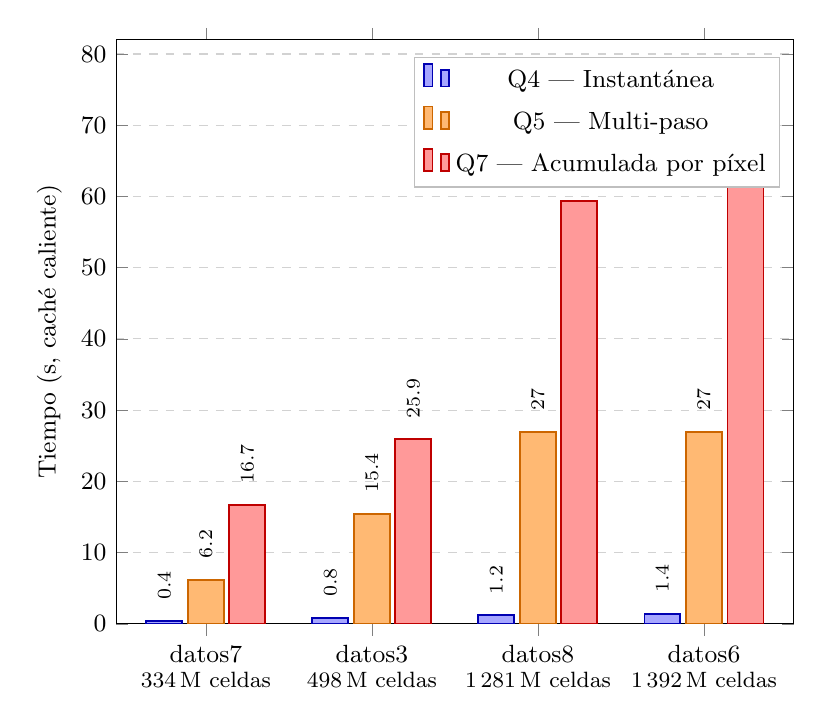
\begin{tikzpicture}
\begin{axis}[
  ybar,
  width=0.84\textwidth,
  height=9cm,
  bar width=13pt,
  enlarge x limits=0.18,
  symbolic x coords={datos7,datos3,datos8,datos6},
  xtick=data,
  xticklabels={
    {datos7\\[-2pt]{\footnotesize 334\,M celdas}},
    {datos3\\[-2pt]{\footnotesize 498\,M celdas}},
    {datos8\\[-2pt]{\footnotesize 1\,281\,M celdas}},
    {datos6\\[-2pt]{\footnotesize 1\,392\,M celdas}}
  },
  xticklabel style={align=center, font=\small},
  ylabel={Tiempo (s, caché caliente)},
  ylabel style={font=\small},
  ymin=0, ymax=82,
  ytick={0,10,20,30,40,50,60,70,80},
  ymajorgrids=true,
  grid style={dashed, gray!35},
  legend style={
    at={(0.98,0.97)}, anchor=north east,
    font=\small, draw=gray!50, fill=white,
    legend columns=1, row sep=3pt
  },
  tick label style={font=\small},
  nodes near coords,
  nodes near coords style={font=\scriptsize, rotate=90, anchor=west, xshift=4pt},
]

\addplot[fill=blue!35, draw=blue!70!black, line width=0.7pt]
    coordinates {(datos7,0.4) (datos3,0.8) (datos8,1.2) (datos6,1.4)};
\addlegendentry{Q4 — Instantánea}

\addplot[fill=orange!55, draw=orange!80!black, line width=0.7pt]
    coordinates {(datos7,6.2) (datos3,15.4) (datos8,27.0) (datos6,27.0)};
\addlegendentry{Q5 — Multi-paso}

\addplot[fill=red!40, draw=red!75!black, line width=0.7pt]
    coordinates {(datos7,16.7) (datos3,25.9) (datos8,59.3) (datos6,69.5)};
\addlegendentry{Q7 — Acumulada por píxel}

\end{axis}
\end{tikzpicture}
\caption{Tiempo de consulta (caché caliente, dominio completo) en cuatro escenarios con distinto número de celdas húmedas. Q4 (instantánea) escala de forma casi plana. Q5 y Q7 crecen de forma aproximadamente lineal con el volumen: al pasar de 334\,M (datos7) a 1\,392\,M celdas (datos6), Q5 se multiplica por 4,4$\times$ y Q7 por 4,2$\times$.}
\label{fig:escalabilidad}
\end{figure}
